\section{Related Work}
The target of this project was to create a newly kickbale and flickable interface used in the outside. For that we firstly did some researches in the web getting inspirated for what we could do.
At least, we hadn't used those literature we had found because there was no interface that can be kicked.
 
\subsection{Listening Lanterns}
The idea of this project was to create a kickable interface for the outside. One of our first findings, was a bubble changing its colour by holding it. The idea of those people was to create a new portable device lightning up your way home in the dark. Firstly, in the middle ages, each person used its own lantern. Later, in the beginning of 18th century some cities like Paris started to lighten their streets at night. They wanted to go back and give each person an own personnel light. So each of those lanterns had an own specifying colour and a fading pattern.\newline
With this basic idea, they started to implement new ideas. \newline

\subsection{DJ Light}

\begin{figure}[h!]
	\centering
	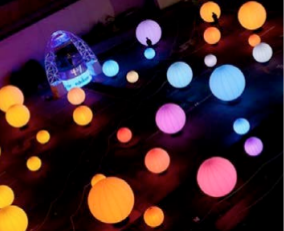
\includegraphics[width=0.5\textwidth, clip=true, keepaspectratio=true]{./pic/dj_light.png}
	\caption{DJ Lights}
	\label{fig:DJ_Lights}
\end{figure}

Using that lantern idea, another team created a public sound and light installation.\newline
They built several sphere - formed devices which can change their colour by different auditive input. With this technology, visitors can perform an own orchestration. Because there are many spheres, the installation can be transported and reinstalled relatively simple. So the devices are pretty good for a usage in the outdoor.\newline
This idea of multiple small devices we used to. \newline 
http://www.wordlesstech.com/2011/01/16/dj-light-installation-video [09.09.2013, 13:50]\newline

\subsection{Throwable Interfaces}
Another very interesting project was to built sticky LED candles which can be threw onto a wall where they rest. After that, an interacting person can target one of those candles with a laser remote. When they get targeted, they changed their color. \newline

\subsection{Urban Cursor}

\begin{figure}[h!]
	\centering
	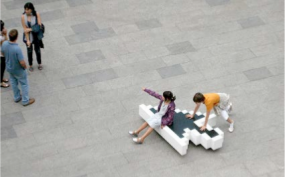
\includegraphics[width=0.5\textwidth, clip=true, keepaspectratio=true]{./pic/urban_cursor.png}
	\caption{Urban Cursor}
	\label{fig:urban_cursor}
\end{figure}

Another urban hci - project we recognized was the Urban Cursor.\newline 
Here, a team created a furniture, designed like a cursor. Approximately, its size is about two to three square metres. The whole thing is easy moveable, because of its wheels. The feature of the cursor is the GPS - tracking system. So the team could determine how the passers - by moved the furniture through the urban space.\newline
The cursor has a very large size because merely people should use it together, so that the project has a social aspect to.
http://www.urbancursor.com [09.09.2013] 

\subsection{Pixels Light Installation}

\begin{figure}[h!]
	\centering
	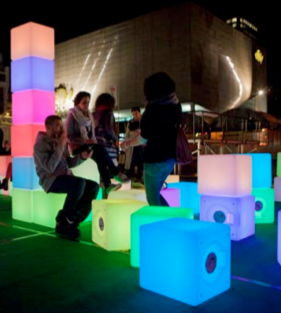
\includegraphics[width=0.5\textwidth, clip=true, keepaspectratio=true]{./pic/pixels_light_installation.png}
	\caption{Pixels Light Installation}
	\label{fig:pixels_light_installation}
\end{figure}
Here the designers built merely cube - devices. \newline
The idea was to built an installation similar to lego \texttrademark where a user can put those devices together or stack them to built different constructed forms. \newline
The cubes are color and intensity changing by rotation. Beyond that, each of the devices is direct and wirelessly connected to the others. So the environment is not driven by a server - client - system.\newline
By using the Arduino technology, those devices are using RF - and IF - sensors, so that they can recognize each other. So when they got kinetic input they will change their colour. With the connection the installation recognizes when some devices are put together, then the construct can be lighten up just in one colour. (All cubes are changing to that one colour.)\newline
 Furthermore the cubes are waterproof, so they can be used in the outside.\newline
\newline
http://www.lightpublic.com/lighting-articles/get-pixelated-with-the-pixels-light-installation [09.09.2013] \newline

\subsection{Liquid bricks}

\begin{figure}[h!]
	\centering
	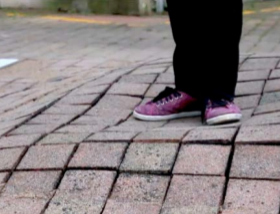
\includegraphics[width=0.5\textwidth, clip=true, keepaspectratio=true]{./pic/liquid_bricks.png}
	\caption{Liquid Bricks}
	\label{fig:liquid_bricks}
\end{figure}
 
This was a small urban project about a water - filled pouch. \newline
The idea was to built any furniture which can be used to make a fun for the passers - by. With this the team designed a texture seeming like the street's bricks. After that, they put the pouch to the ground - level of the street / square. So when a person was walking over it, it seemed like walking over a inconsistent place.\newline
\newline
http://www.thisiscolossal.com/2011/06/liquid-bricks\newline

\subsection{21 swings}

\begin{figure}[h!]
	\centering
	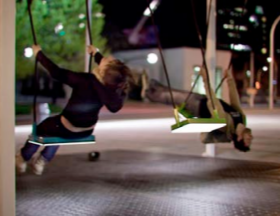
\includegraphics[width=0.5\textwidth, clip=true, keepaspectratio=true]{./pic/21_swings.png}
	\caption{21 Swings}
	\label{fig:21_swings}
\end{figure}

In Montreal a gigantic wings installation was created along a street.\newline
By swinging on a swing a music note is played. So when just one lonely passer - by is swinging, the system doesn't makes that fun. But when merely users are in action with the swings a hazard harmonic is in creation. \newline
Here the designers used the diatonic music system. This is the system which is known from playing harmonica: When the user is blowing in one specific hole, a tone will sound. When the user is suck in the same hole, the next tone in the musical scale will sound. Here in this project, each swing just gives one tone. It doesn't matter if the swing is swinging back- or forwards. The clue on this pattern is, that there cannot be any false note which doesn't match to the others.\newline
\newline
http://www.fastcodedesign.com/1672192/watch-a-musical-swingset-forms-a-21-piece-orchestra.                
